\chapter{От мод импульса к локальным квантовым полям}

Что такое квантовое поле и как оно связано с частицами? Основным математическим инструментом служит гармонический осциллятор. Поле содержит много возможных мод колебаний, и квантование поля сводится к сопоставлению каждой моде одного квантового гармонического осциллятора. Эту конструкцию проще всего сначала увидеть в конечном периодическом пространстве, где разрешённые моды образуют дискретный набор.

\section{Периодическое пространство и разрешённые волновые числа}

Возьмём одну пространственную координату \(x\) и отождествим точки, разделённые расстоянием \(L\). Такое пространство можно представлять себе как окружность длины \(L\). Это полезный приём конечного объёма. На конечном интервале с концами бегущая волна отражается от концов. На периодическом интервале она может продолжаться в любом из двух направлений без отражения. Симметрия относительно переносов, а следовательно и сохранение импульса, сохраняется, тогда как сложности бесконечного объёма временно устраняются.

Плоская волна имеет вид
\begin{equation}
e^{ikx}.
\end{equation}
После одного обхода по окружности она должна вернуться к своему исходному значению. Поскольку волна равна \(1\) при \(x=0\), периодичность требует
\begin{equation}
e^{ikL}=1.
\end{equation}
Почему это условие выполняется, если взять целое кратное \(2\pi\)? Формула Эйлера даёт
\begin{align}
e^{i2\pi n}
&=\cos(2\pi n)+i\sin(2\pi n)\\
&=1,
\qquad n\in\mathbb Z.
\end{align}
Косинус равен \(1\), а синус равен \(0\) после любого целого числа циклов. Следовательно,
\begin{equation}
kL=2\pi n,
\qquad
k=\frac{2\pi n}{L},
\qquad n\in\mathbb Z.
\end{equation}
Величина \(k\) есть волновое число. Целое число \(n\) нумерует разрешённое волновое число; оно пока не считает частицы.

То же самое условие можно выразить через длину волны. Длина волны — это расстояние, на котором фаза продвигается на один полный цикл, так что
\begin{equation}
k\lambda=2\pi,
\qquad
k=\frac{2\pi}{\lambda}.
\end{equation}
Большой длине волны соответствует малое волновое число, а малой длине волны — большое волновое число. Условие периодичности утверждает, что по окружности укладывается целое число длин волн.

Для квантовомеханической волны импульс равен
\begin{equation}
p=\frac{h}{\lambda}
=\frac{2\pi\hbar}{\lambda}
=\hbar k.
\end{equation}
Таким образом, \(k\) и \(p\) различаются только множителем \(\hbar\). Положительные и отрицательные \(k\) описывают волны, распространяющиеся в противоположных направлениях, и частицы с противоположно направленными импульсами. В единицах, где \(\hbar=1\), \(k\) часто без дополнительных оговорок называют импульсом.

Для каждого разрешённого \(k\) в этой моде может находиться некоторое число квантов. Это вводит второе целое число:
\begin{equation}
n(k)=\text{number of quanta with wave number }k.
\end{equation}
Оно называется числом заполнения. Целое число в \(k=2\pi n/L\) нумерует моду; \(n(k)\) показывает, сколько частиц находится в этой моде. Числа заполнения должны быть заданы и для отрицательных, и для положительных \(k\).

\begin{classroomqa}
\lecturetimestamp{00:11:58}
\audiencequestion{Само \(k\) — целое число?}
\lecturerresponse{Нет. Волновое число является целым кратным \(2\pi/L\): \(k=2\pi n/L\). Целое число \(n\) в этой формуле нумерует разрешённое значение импульса и отлично от числа заполнения \(n(k)\), которое считает кванты в моде.}
\end{classroomqa}

\section{Состояния с заданными числами заполнения и операторы мод}

Квантовое состояние есть вектор, или линейный элемент. Векторы состояния можно складывать и умножать на числа, а операторы действуют на них, порождая другие векторы состояния. Наблюдаемые вещественные величины представлены эрмитовыми операторами. Эти элементарные факты здесь важны, потому что и многочастичное состояние, и поле будут строиться из линейных комбинаций и операторов.

Пусть
\begin{equation}
k_j=\frac{2\pi j}{L},
\qquad j\in\mathbb Z.
\end{equation}
Удобно обозначать многочастичное состояние всей последовательностью чисел заполнения. Используя сокращение \(n_j\equiv n(k_j)\) для записанных элементов, запишем
\begin{equation}
\big|\{n(k_j)\}\big\rangle
=
\big|\ldots,n_{-2},n_{-1},n_0,n_1,n_2,\ldots\big\rangle.
\end{equation}
Элемент \(n(k_1)\) есть число частиц в первой моде с положительным импульсом, \(n(k_2)\) — число частиц во второй и так далее. Эта последовательность продолжается без конца в обе стороны.

\begin{figure}[t]
\centering
\includegraphics[width=0.72\textwidth]{lecture_03_figure_02.png}
\caption{Число заполнения \(n(k)\) для разрешённой импульсной моды.}
\lectureframe{00:15:04}
\end{figure}

Каждая импульсная мода представляет собой гармонический осциллятор. Поэтому у неё есть оператор повышения и оператор понижения. Обозначения, первоначально записанные как \(a^{+}(k)\) и \(a^{-}(k)\), далее будем записывать как \(a^\dagger(k)\) и \(a(k)\). Их действие таково:
\begin{align}
a^\dagger(k)\big|\ldots,n(k),\ldots\big\rangle
&=
\sqrt{n(k)+1}\notag\\
&\quad{}\times
\big|\ldots,n(k)+1,\ldots\big\rangle,
\\
a(k)\big|\ldots,n(k),\ldots\big\rangle
&=
\sqrt{n(k)}\,
\big|\ldots,n(k)-1,\ldots\big\rangle.
\end{align}
Оператор \(a^\dagger(k)\) обращается к ячейке, соответствующей \(k\), увеличивает это число заполнения на единицу и умножает состояние на \(\sqrt{n(k)+1}\). Оператор \(a(k)\) уменьшает то же число заполнения на единицу и даёт множитель \(\sqrt{n(k)}\). Для каждого разрешённого импульса имеется одна такая пара.

\begin{figure}[t]
\centering
\includegraphics[width=0.58\textwidth]{lecture_03_figure_03.png}
\caption{Операторы рождения и уничтожения, связанные с импульсной модой \(k\).}
\lectureframe{00:17:14}
\end{figure}

\section{Коэффициенты Фурье становятся операторами}

Связь между этими операторами осциллятора и полем начинается с обычного классического ряда Фурье. Комплексное классическое поле на периодическом интервале можно записать в виде
\begin{align}
\psi(x)&=\sum_k \alpha(k)e^{ikx},\\
\psi^*(x)&=\sum_k \alpha^*(k)e^{-ikx},
\end{align}
где в каждой сумме перебираются разрешённые значения \(k=2\pi n/L\). Это эквивалентно разложению поля по синусам и косинусам.

Комплексное поле имеет вещественную и мнимую части. Его комплексное сопряжение меняет знак мнимой части, и \(e^{ikx}\) переходит в \(e^{-ikx}\). Задание всех коэффициентов \(\alpha(k)\) задаёт классическое поле. Нет необходимости независимо задавать \(\alpha^*(k)\) после того, как известно \(\alpha(k)\), но вещественная и мнимая части каждого коэффициента являются отдельными вещественными величинами. Их можно измерять как амплитуды соответствующих компонент Фурье. В этом смысле один комплексный коэффициент объединяет две классические наблюдаемые величины.

Квантование заменяет эти классические коэффициенты Фурье операторами. Обычный знак равенства отождествлял бы объекты разной природы, поэтому лучше записать правило замены:
\begin{equation}
\alpha(k)\rightsquigarrow a(k),
\qquad
\alpha^*(k)\rightsquigarrow a^\dagger(k).
\end{equation}
При согласованном выборе знаков Фурье квантовые поля определяются так:
\begin{align}
\Psi(x)&=\sum_k a(k)e^{ikx},\\
\Psi^\dagger(x)&=\sum_k a^\dagger(k)e^{-ikx}.
\end{align}
\editorialnote{В устном объяснении соглашение о знаках Фурье меняется, а позднее даже ставится под вопрос. Сопряжённая пара, используемая здесь, — это соглашение, которое видно в более ясном разложении поля и в вычислении состояния положения: \(\Psi\) содержит \(e^{ikx}\), а \(\Psi^\dagger\) содержит \(e^{-ikx}\). Если последовательно обратить все знаки, получится та же самая конструкция.}

На данный момент это определение: квантовое поле — это сумма Фурье, коэффициентами которой служат операторы. Более полное обоснование должно было бы показать, как эти операторы воспроизводят классические коэффициенты в подходящем пределе, а для этого нужна некоторая динамика. Этот вопрос откладывается. Уже сейчас ясно, что само поле является оператором, а соотношения между его коэффициентами Фурье — это соотношения рождения и уничтожения для гармонических осцилляторов.

\begin{classroomqa}
\lecturetimestamp{00:26:48}
\audiencequestion{Означает ли введение операторов рождения и уничтожения, что динамика обязательно создаёт и уничтожает частицы?}
\lecturerresponse{Нет. Эти операторы — математические операции, меняющие числа заполнения. Вопрос о том, меняют ли законы природы число частиц на самом деле, относится к динамике. Если динамика допускает такие изменения, эти операторы дают естественный язык для их описания.}
\end{classroomqa}

\section{Рассеяние и переменное число частиц}

Сначала рассмотрим процесс, который не меняет числа частиц. Предположим, что единственная частица, присутствующая вначале, имеет импульс \(k_7\). В обозначениях чисел заполнения её состояние содержит \(1\) в седьмой ячейке и нули во всех остальных:
\begin{equation}
|k_7\rangle
=
|\ldots,0,\underset{k_7}{1},0,\ldots\rangle.
\end{equation}
Процесс рассеяния меняет её импульс с \(k_7\) на \(k_9\). Оператор, осуществляющий именно такое изменение, имеет вид
\begin{equation}
a^\dagger(k_9)a(k_7).
\end{equation}
Крайний справа оператор действует первым: он удаляет частицу из ячейки \(k_7\). Затем левый оператор создаёт частицу в ячейке \(k_9\).

\begin{classroomqa}
\lecturetimestamp{00:31:37}
\audiencequestion{Откуда в процессе \(k_7\to k_9\) берутся множители с квадратным корнем?}
\lecturerresponse{Множитель при уничтожении равен \(\sqrt{n(k_7)}=\sqrt{1}=1\). После этого удаления система оказывается в состоянии из одних нулей. Поскольку мода \(k_9\) пуста, множитель при рождении равен \(\sqrt{n(k_9)+1}=\sqrt{1}=1\). Поэтому ни один из них не изменяет численный коэффициент в этом одночастичном примере.}
\end{classroomqa}

Выполним теперь оба шага. Уничтожение даёт
\begin{align}
a(k_7)|k_7\rangle
&=
\sqrt{1}\,|\ldots,0,0,0,\ldots\rangle\\
&=|0\rangle.
\end{align}
Состояние из одних нулей есть вакуум. Это состояние без частиц, и в этой простой совокупности осцилляторов оно также является основным состоянием. Рождение в пустой моде \(k_9\) затем даёт
\begin{equation}
a^\dagger(k_9)|0\rangle
=\sqrt{0+1}\,|k_9\rangle
=|k_9\rangle.
\end{equation}
Следовательно,
\begin{equation}
a^\dagger(k_9)a(k_7)|k_7\rangle=|k_9\rangle.
\end{equation}
По ячейкам видно, что единственная \(1\) просто переместилась из седьмой импульсной моды в девятую. Поскольку ни одно число заполнения ни разу не превысило единицы, оба множителя с квадратным корнем были равны единице. Они станут важны, как только будет задействована уже занятая мода.

Этот процесс «один в один» можно было бы описать и в обычной одночастичной квантовой механике: одна частица меняет свой импульс. Язык чисел заполнения становится незаменимым, когда число частиц может изменяться. Например,
\begin{equation}
a^\dagger(k_9)a^\dagger(k_{16})a(k_7)|k_7\rangle
=|k_9,k_{16}\rangle
\end{equation}
описывает математический переход от одной входящей частицы в моде \(k_7\) к двум исходящим частицам, одной в \(k_9\) и одной в \(k_{16}\). Мишень может поглотить входящую частицу, испустить две исходящие частицы и воспринять любую необходимую отдачу. Такой процесс нельзя представить в гильбертовом пространстве, ограниченном одной частицей, но он естественно укладывается в пространство состояний, в котором числа заполнения могут изменяться. Само по себе это операторное выражение не является законом природы; это язык, на котором можно записать закон, изменяющий число частиц.

\section{Оператор поля в точке}

Что создает оператор \(\Psi^\dagger(x)\) в координатном пространстве? Квантовые состояния образуют линейное пространство: состояния с определенным импульсом можно складывать с комплексными коэффициентами, образуя новое состояние. Начнем с вакуума. Поскольку каждая мода пуста,
\begin{equation}
\Psi(x)|0\rangle=0.
\end{equation}
Нуль справа — это нулевой вектор: оператор уничтожения не может найти ни одной частицы, которую можно было бы убрать.

Сопряженное поле действует иначе:
\begin{align}
\Psi^\dagger(x)|0\rangle
&=\sum_k e^{-ikx}a^\dagger(k)|0\rangle\\
&=\sum_k e^{-ikx}|k\rangle,
\end{align}
где
\begin{equation}
|k\rangle=a^\dagger(k)|0\rangle
\end{equation}
— одночастичное состояние с импульсом \(\hbar k\).

\begin{figure}[t]
\centering
\includegraphics[width=0.70\textwidth]{lecture_03_figure_05.png}
\caption{Формальное состояние в координатном пространстве \(\Psi^\dagger(x)|0\rangle\), разложенное по одночастичным импульсным состояниям.}
\lectureframe{00:43:16}
\end{figure}

Формально и с точностью до нормировки эта сумма представляет собой обобщенное координатное состояние одночастичной квантовой механики.\footnote{При бесконечном числе импульсных мод точно локализованное координатное состояние ненормируемо. Если вместо этого ввести конечное обрезание по импульсу и нормировать усеченную сумму, получится резко локализованный волновой пакет с центром в \(x\).} Собственные состояния импульса, взятые с коэффициентами \(e^{-ikx}\), обеспечивают локализацию в \(x\). В этом формальном смысле,
\begin{equation}
\Psi^\dagger(x)\ \text{creates a particle at position }x,
\end{equation}
тогда как
\begin{equation}
\Psi(x)\ \text{annihilates a particle at position }x.
\end{equation}
Оператор моды \(a^\dagger(k)\) создает частицу с определенным импульсом. Оператор поля \(\Psi^\dagger(x)\) создает когерентную суперпозицию допустимых состояний с определенным импульсом, формально локализованную в \(x\).

В формальной ненормированной сумме каждый коэффициент \(e^{-ikx}\) имеет модуль единица. При конечном обрезании нормированное усеченное состояние имеет коэффициенты одинакового модуля для оставленных импульсов, а их фазы создают волновой пакет, резко локализованный вблизи \(x\). Это элементарная связь между квантовым полем и частицами.

Если пока не учитывать осложнения специальной теории относительности, \(\Psi^\dagger(x)\) в этой модели создает частицу в точке \(x\). Для релятивистских полей требуются уточнения, но разложение Фурье с операторными коэффициентами и различие между операторами импульсных мод и операторами в координатном пространстве остаются основополагающими.

\begin{classroomqa}
\lecturetimestamp{00:44:59}
\audiencequestion{Является ли \(x\) точкой на периодической окружности, и что происходит, когда окружность становится большой?}
\lecturerresponse{Да. В конечной модели \(x\) — точка на окружности. Соседние допустимые волновые числа отделены интервалом \(2\pi/L\). По мере увеличения \(L\) этот интервал уменьшается, так что для любого заданного импульса существует допустимое значение, сколь угодно близкое к нему. В пределе бесконечного объема суммы по \(k\) заменяются интегралами по \(k\). Полезно сначала понять дискретные суммы.}
\end{classroomqa}

\section{Локальные реакции частиц}

После того как \(\Psi(x)\) и \(\Psi^\dagger(x)\) интерпретированы как операторы уничтожения и рождения частиц в точке, локальность можно выразить непосредственно. Представьте, что частица поглощается мишенью, резко локализованной в \(x\), тогда как одна исходящая частица внезапно появляется возле Alpha Centauri, а другая — возле Betelgeuse. Такая реакция нелокальна: ее разнесенные события не могут быть связаны обычным распространением.

Можно было бы сперва ослабить это требование и разрешить, чтобы исходящие частицы испускались где-то в малой области вокруг мишени. Строгая локальная идеализация сильнее: если входящая частица поглощается в \(x\), то исходящие частицы создаются в той же самой точке. Использование полей, взятых в разнесенных точках, описывало бы вместо этого нелокальное произведение операторов. Поэтому локальная операция «один в два» имеет вид
\begin{equation}
\Psi^\dagger(x)\Psi^\dagger(x)\Psi(x).
\end{equation}
Крайнее справа поле уничтожает входящую частицу в \(x\); два поля слева от него создают там две исходящие частицы.\footnote{Локальная схема «один в два» соответствует реакции, описанной в 00:47:38--00:49:13.}

\begin{figure}[t]
\centering
\begin{tikzpicture}[scale=1.0]
\draw[->] (-2.2,0) -- (0,0);
\fill (0,0) circle (2.2pt);
\draw[->] (0,0) -- (2.0,1.1);
\draw[->] (0,0) -- (2.0,-1.1);
\node at (-1.25,0.3) {$k_{\mathrm{initial}}$};
\node[right] at (0.05,0.05) {$x$};
\node at (1.48,1.34) {$\ell$};
\node at (1.48,-1.34) {$m$};
\end{tikzpicture}
\caption{Одна входящая частица поглощается в \(x\), и две исходящие частицы создаются в той же точке.}
\end{figure}

Пусть входящее состояние содержит одну частицу с определенным волновым числом \(k_{\mathrm{initial}}\). Чтобы определить исходящие импульсы, подставим импульсные разложения локальных полей. Важно отделять фиксированную метку импульса от немого индекса суммирования. Запишем
\begin{align}
\Psi(x)&=\sum_q a(q)e^{iqx},\\
\Psi^\dagger(x)&=\sum_\ell a^\dagger(\ell)e^{-i\ell x}.
\end{align}
Индекс \(q\) суммируется, тогда как \(k_{\mathrm{initial}}\) обозначает конкретную занятую входящую моду. Две копии \(\Psi^\dagger(x)\) также требуют независимых немых индексов, скажем \(\ell\) и \(m\). Повторное использование одного индекса неверно связало бы две независимые суммы. Здесь \(\ell\) и \(m\) — волновые числа; \(m\) не обозначает массу.

Наглядная картина — фотон, налетающий на атом, локализованный в \(x\), после чего из этой точки вылетают два фотона. Простое поле, используемое здесь, лучше подходит для нерелятивистских частиц, чем для полностью релятивистского фотонного поля, так что язык фотонов служит лишь для иллюстрации учета операторов.

Поле уничтожения действует первым:
\begin{align}
\Psi(x)|k_{\mathrm{initial}}\rangle
&=\sum_q e^{iqx}a(q)a^\dagger(k_{\mathrm{initial}})|0\rangle.
\end{align}
Все члены обращаются в нуль, кроме члена с \(q=k_{\mathrm{initial}}\). Оператор уничтожения должен найти частицу в собственной моде. Поэтому
\begin{equation}
\Psi(x)|k_{\mathrm{initial}}\rangle
=e^{ik_{\mathrm{initial}}x}|0\rangle.
\end{equation}
Два поля рождения затем дают
\begin{align}
&\Psi^\dagger(x)\Psi^\dagger(x)\Psi(x)
|k_{\mathrm{initial}}\rangle
\\
&\quad=
e^{ik_{\mathrm{initial}}x}
\sum_{\ell,m}
e^{-i\ell x}e^{-imx}
a^\dagger(\ell)a^\dagger(m)|0\rangle
\\
&\quad=
\sum_{\ell,m}
e^{i(k_{\mathrm{initial}}-\ell-m)x}
a^\dagger(\ell)a^\dagger(m)|0\rangle.
\end{align}
При неравных \(\ell\) и \(m\) операторное состояние можно обозначить как \(|\ell,m\rangle\): каждая из двух мод занята одной частицей. Итоговый результат — сумма по всем таким двухчастичным конфигурациям импульсов, с фазой, определяемой входящим и исходящими импульсами.

\begin{classroomqa}
\lecturetimestamp{01:00:36}
\audiencequestion{Коммутируют ли два оператора рождения?}
\lecturerresponse{Да. Все операторы рождения коммутируют друг с другом, и все операторы уничтожения коммутируют друг с другом. Оператор рождения и оператор уничтожения коммутируют, когда они относятся к разным модам; для одной и той же моды их коммутатор ненулевой.}
\end{classroomqa}

\begin{classroomqa}
\lecturetimestamp{01:01:34}
\audiencequestion{Должны ли два исходящих импульса удовлетворять закону сохранения импульса?}
\lecturerresponse{Показанные частицы сами по себе не обязаны сохранять импульс, потому что атом или мишень может испытать отдачу. Разность \(k_{\mathrm{initial}}-\ell-m\) — это импульс, переданный мишени. Сохраняющейся величиной является полный импульс, включая мишень.}
\end{classroomqa}

Поскольку коэффициент \(e^{i(k_{\mathrm{initial}}-\ell-m)x}\) представляет собой чистую фазу, его модуль равен единице. На первый взгляд это предполагает одинаковые вероятностные веса для всех пар \((\ell,m)\). Однако важная оговорка возникает, когда две метки совпадают.

Если \(\ell=m\), первый оператор рождения помещает одну частицу в моду \(m\), а второй действует на моду, уже занятую один раз:
\begin{align}
a^\dagger(m)a^\dagger(m)|0\rangle
&=a^\dagger(m)|1_m\rangle\\
&=\sqrt{2}\,|2_m\rangle.
\end{align}
Таким образом, двойное создание в одной моде имеет дополнительную амплитуду \(\sqrt{2}\). Возведение амплитуды в квадрат дает в вероятности множитель \(2\).

\begin{classroomqa}
\lecturetimestamp{01:04:54}
\audiencequestion{Должны ли \(\ell\) и \(m\) отличаться на единицу, потому что коэффициент рождения содержит \(n+1\)?}
\lecturerresponse{Нет. Символы \(\ell\) и \(m\) обозначают импульсные моды. \(n\) в \(\sqrt{n+1}\) — это число заполнения конкретной моды, на которую действует оператор рождения. Метки импульса и числа частиц — разные целые числа.}
\end{classroomqa}

\begin{figure}[t]
\centering
\includegraphics[width=0.92\textwidth]{lecture_03_figure_06.png}
\caption{Разложение в импульсном пространстве локальной амплитуды перехода одной частицы в две.}
\lectureframe{01:05:44}
\end{figure}

Частицы в этой конструкции тождественны. Следовательно, \(\sqrt{2}\) — бозонный фактор заполнения, а не метка, отличающая первую частицу от второй. Если его возвести в квадрат, то на первый взгляд получается, что исход с одинаковыми импульсами вдвое вероятнее одного отдельного члена с различными импульсами. К этому сравнению нужно будет вернуться, когда члены в двойной сумме будут аккуратно подсчитаны.

\begin{classroomqa}
\lecturetimestamp{01:06:43}
\audiencequestion{В сложной реакции как выбирают порядок операторов рождения и уничтожения?}
\lecturerresponse{Выражение, в котором все операторы рождения стоят слева, а все операторы уничтожения справа, называется нормально упорядоченным. В такой форме крайние справа операторы сначала уничтожают входящие частицы, а оставшиеся операторы создают исходящие частицы.}
\end{classroomqa}

Перестановка смешанной пары операторов рождения--уничтожения, вообще говоря, не сводится к простой перестановке: необходимо использовать коммутатор, и для одной и той же моды это дает дополнительный член.\footnote{Это уточнение о коммутаторе представляет собой редакторское исправление неформального обсуждения нормального упорядочения в 01:06:43.}

\begin{classroomqa}
\lecturetimestamp{01:07:30}
\audiencequestion{Если все импульсные амплитуды имеют одинаковый модуль, что означает утверждение вроде ``вдвое более вероятно''?}
\lecturerresponse{Помните о конечной полости. Допустимые в ней импульсы дискретны, так что вероятности можно сравнивать по модам. Сравнение ведется не между вероятностями изолированных точек в континууме.}
\end{classroomqa}

При \(\ell\ne m\) неограниченная двойная сумма содержит оба упорядоченных члена
\begin{equation}
a^\dagger(\ell)a^\dagger(m)|0\rangle
\quad\text{and}\quad
a^\dagger(m)a^\dagger(\ell)|0\rangle.
\end{equation}

\begin{classroomqa}
\lecturetimestamp{01:08:24}
\audiencequestion{Когда \(\ell\ne m\), не возникает ли одно и то же конечное состояние дважды в двойной сумме, один раз как \((\ell,m)\) и один раз как \((m,\ell)\)?}
\lecturerresponse{Да. Если \(\ell\ne m\), то присутствуют оба члена, \((\ell,m)\) и \((m,\ell)\), и поскольку операторы рождения коммутируют, они описывают одно и то же физическое состояние.}
\end{classroomqa}

Два упорядоченных члена равны, поэтому, прежде чем проводить количественное сравнение каналов, нужно учесть нормировку состояний и этот двойной счет. Надежный алгебраический вывод здесь более узок, и для дальнейшего этого достаточно: создание частицы в моде, уже занятой \(n\) тождественными бозонами, дает множитель \(\sqrt{n+1}\).

\section{Спонтанное и вынужденное излучение}

Более ясный пример выделяет корневой множитель. Предположим, что объект, локализованный в \(x\), испускает один фотон. Если фотонное поле изначально находится в вакууме, то исходящее состояние равно
\begin{align}
\Psi^\dagger(x)|0\rangle
&=\sum_k e^{-ikx}a^\dagger(k)|0\rangle\\
&=\sum_k e^{-ikx}|k\rangle.
\end{align}
В рамках этой упрощенной модели все импульсы имеют одинаковый модуль амплитуды. Когда фотонов заранее нет, излучение является спонтанным.

Теперь предположим, что в моде \(\ell\) уже есть один фотон. Действие того же локального поля рождения дает два типа членов:
\begin{equation}
\Psi^\dagger(x)|\ell\rangle
=
\sum_{k\ne\ell}e^{-ikx}|k,\ell\rangle
+e^{-i\ell x}\sqrt{2}\,|2_\ell\rangle.
\end{equation}
При \(k\ne\ell\) оператор создает фотон в пустой моде, поэтому коэффициент равен \(\sqrt{0+1}=1\). При \(k=\ell\) он создает его в занятой моде, поэтому коэффициент равен \(\sqrt{1+1}=\sqrt{2}\). Исходный фотон здесь лишь присутствует; новый фотон предпочтительно испускается в уже занятую им моду.

\begin{classroomqa}
\lecturetimestamp{01:16:14}
\audiencequestion{Должен ли уже существующий фотон находиться в том же месте, чтобы стимулировать излучение?}
\lecturerresponse{Это упрощенное вычисление относится к заселенности одной и той же импульсной моды, а не к двум частицам в одном точно определенном положении. Частица не может иметь одновременно точное положение и точный импульс. Реальные фотоны описываются волновыми пакетами, тогда как идеализация с полостью дает определенные дискретные моды. В этой постановке усиление происходит в уже занятую моду полости.}
\end{classroomqa}

Если мода \(\ell\) вначале содержит \(n_\ell\) фотонов, то
\begin{equation}
a^\dagger(\ell)
|\ldots,n_\ell,\ldots\rangle
=
\sqrt{n_\ell+1}
\,|\ldots,n_\ell+1,\ldots\rangle.
\end{equation}
Следовательно, вероятность усиливается в \(n_\ell+1\) раз. Если уже имеется один фотон, множитель равен \(2\). Если в моде сто фотонов, то амплитудный множитель равен \(\sqrt{101}\), а вероятность испускания в эту моду в \(101\) раз больше, чем для пустой моды. Чем больше квантов уже находится в бозонной моде, тем вероятнее, что следующий квант будет испущен в эту моду. Это и есть вынужденное излучение.

Тот же эффект заселенности проявляется и в реакциях рассеяния. Если столкновение может породить частицу в нескольких модах, уже имеющаяся заселенность усиливает рождение в занятые моды. Это общее свойство данной осцилляторной алгебры, а не особая черта атомного распада.

\begin{classroomqa}
\lecturetimestamp{01:18:15}
\audiencequestion{В рассмотренном ранее двухчастичном процессе имеют ли две вновь создаваемые частицы больший вес и тогда, когда их импульсы различны?}
\lecturerresponse{Да. В упорядоченной двойной сумме пара с разными импульсами встречается в двух порядках. Множитель для одной и той же моды \(\sqrt{2}\) уменьшает это комбинаторное различие, но сам по себе его не устраняет.}
\end{classroomqa}

Как и раньше, для физического сравнения каналов по-прежнему требуются согласованные нормировка состояний и подсчет.

\begin{classroomqa}
\lecturetimestamp{01:18:30}
\audiencequestion{Значит ли это, что бозоны притягиваются к уже занятым состояниям импульса?}
\lecturerresponse{Нет. Никакой буквальной силы или притяжения здесь нет. Усиление является статистическим следствием тождественности частиц и корневых множителей в бозонных операторах рождения.}
\end{classroomqa}

Полезно различать эти два названия. Если фотонов нет, то в коэффициенте стоит \(n=0\), что дает единичный множитель, связанный со спонтанным излучением. Если фотоны уже присутствуют, то множитель \(n+1\) делает излучение в их моду более вероятным; это и есть вынужденное излучение.

Существует классический аналог. Уже существующая электромагнитная волна, проходящая мимо атома, приводит в движение его электроны. Электроны, приводимые ею в движение, излучают сильнее, чем без волны, а добавочное излучение следует направлению и волновому числу возбуждающей волны. В квантовом утверждении уже существующая волна заменяется заселенными фотонными модами: имеющиеся кванты стимулируют рождение новых квантов в той же моде.

Частицы, подчиняющиеся этой алгебре гармонического осциллятора, являются бозонами. У них есть статистическая тенденция накапливаться в занятых состояниях, хотя они не притягивают друг друга в эти состояния. Частицы бывают двух статистических типов: бозоны и фермионы. Рассматриваемая здесь конструкция бозонная; противоположное, фермионное поведение будет рассмотрено позже.

\section{Бозонная алгебра и плотность частиц}

Для каждой импульсной моды существуют операторы рождения и уничтожения. Их алгебра имеет вид
\begin{align}
[a^\dagger(k),a^\dagger(\ell)]&=0,\\
[a(k),a(\ell)]&=0,\\
[a(k),a^\dagger(\ell)]&=\delta_{k\ell}.
\end{align}
Здесь
\begin{equation}
[A,B]=AB-BA,
\end{equation}
а дельта Кронекера равна
\begin{equation}
\delta_{k\ell}=
\begin{cases}
1,&k=\ell,\\
0,&k\ne\ell.
\end{cases}
\end{equation}
Операторы рождения коммутируют как при равных, так и при неравных импульсах; то же верно и для операторов уничтожения. Смешанная пара коммутирует при различных импульсах; при одном и том же импульсе она имеет привычный коммутатор одиночного осциллятора.

Вместе с фурье-определением \(\Psi(x)\) эти соотношения задают простейшее бозонное квантовое поле. Назначение этого поля — создавать и уничтожать частицы, по модам или в заданных положениях.

Рассмотрим теперь оператор
\begin{equation}
\int_0^L dx\,\Psi^\dagger(x)\Psi(x).
\end{equation}
Вместо того чтобы заранее называть его, вычислим, что он собой представляет. Подстановка фурье-разложений дает
\begin{align}
\int_0^L dx\,\Psi^\dagger(x)\Psi(x)
&=
\sum_{k,\ell}a^\dagger(k)a(\ell)
\int_0^L dx\,e^{-ikx}e^{i\ell x}
\\
&=
\sum_{k,\ell}a^\dagger(k)a(\ell)
\int_0^L dx\,e^{i(\ell-k)x}.
\end{align}
Если \(k=\ell\), экспонента равна \(1\), а интеграл равен \(L\). Если \(k\ne\ell\), то по окружности интегрируется целое число периодов синуса и косинуса; положительные и отрицательные части взаимно сокращаются. Таким образом,
\begin{equation}
\int_0^L dx\,e^{i(\ell-k)x}=L\delta_{k\ell}.
\end{equation}
Двойная сумма сводится к
\begin{equation}
\int_0^L dx\,\Psi^\dagger(x)\Psi(x)
=L\sum_k a^\dagger(k)a(k).
\end{equation}
Для каждой моды
\begin{equation}
a^\dagger(k)a(k)=N_k
\end{equation}
есть оператор числа заполнения. Суммирование по всем модам дает число всех частиц:
\begin{equation}
N=\sum_k N_k=\sum_k a^\dagger(k)a(k).
\end{equation}
При используемой здесь фурье-нормировке
\begin{equation}
N=\frac{1}{L}\int_0^L dx\,
\Psi^\dagger(x)\Psi(x).
\end{equation}
В других соглашениях множители типа \(1/\sqrt{L}\) включают в фурье-разложение и убирают явный множитель \(1/L\) здесь. В используемом соглашении локальный оператор плотности частиц имеет вид
\begin{equation}
\rho(x)=\frac{1}{L}\Psi^\dagger(x)\Psi(x),
\qquad
\int_0^L dx\,\rho(x)=N.
\end{equation}
Следовательно, \(\Psi^\dagger(x)\Psi(x)\) пропорционально плотности частиц. Называть это числом частиц в одной математической точке было бы вводящим в заблуждение; подходящим локальным понятием является плотность.

Полное число частиц может сохраняться, а может и не сохраняться. Если динамика создает или поглощает частицы, \(N\) может меняться со временем. Если число частиц сохраняется данной динамикой, то \(N\) является сохраняемой наблюдаемой.

Зная коммутаторы модовых операторов, можно также вычислить коммутаторы \(\Psi(x)\) и \(\Psi^\dagger(x)\). Это вычисление оставляется в качестве полезного упражнения на применение фурье-сумм.

Эта конструкция описывает один вид тождественных бозонов. Под тождественностью здесь понимается, что все частицы относятся к одному и тому же виду, хотя их положения и импульсы могут различаться. Нельзя помещать электроны и фотоны в одно и то же поле \(\Psi\). Поле фотона требует релятивистских уточнений этой элементарной модели. Поле электрона требует другой, фермионной алгебры.

\begin{classroomqa}
\lecturetimestamp{01:35:43}
\audiencequestion{Является ли эта конструкция только одномерной?}
\lecturerresponse{До сих пор в примере была одна пространственная координата, но ничего существенного от этого не зависит. Более высокие размерности получаются введением дополнительных координат и компонент импульса.}
\end{classroomqa}

\editorialnote{Краткий обмен репликами здесь, по-видимому, начинается с флуоресценции и вынужденного излучения, а затем переходит к прозрачности и интерференции. Поврежденная формулировка не позволяет надежно восстановить ни вопрос, ни ответ.}

Примеры включают фотоны, бозон Хиггса и гравитоны.\footnote{Другие названия частиц в кратком перечне примеров неразборчивы и поэтому не сохраняются.}

\section{Большая заселенность и предел классического поля}

Комплексный полевой оператор сам по себе не является одной эрмитовой наблюдаемой. Его две эрмитовы компоненты имеют вид
\begin{equation}
\Psi_1(x)=\frac{\Psi(x)+\Psi^\dagger(x)}{2},
\quad
\Psi_2(x)=\frac{\Psi(x)-\Psi^\dagger(x)}{2i}.
\end{equation}
Они являются квантовыми аналогами действительной и мнимой частей классического поля. Они не коммутируют, поэтому обе нельзя одновременно измерить с произвольной точностью. Это полевой вариант неопределённости между сопряжёнными переменными гармонического осциллятора.

Когда же поле может вести себя как классическая волна? Рассмотрим одну сильно возбуждённую импульсную моду \(k\). Её оператор числа имеет вид
\begin{equation}
a^\dagger(k)a(k)=N_k.
\end{equation}
Предположим, что в состоянии велико среднее число заполнения, \(\langle N_k\rangle=n_k\gg 1\). Тогда масштаб, доступный для макроскопической амплитуды осциллятора, имеет порядок \(\sqrt{n_k}\). Между тем правая часть
\begin{equation}
[a(k),a^\dagger(k)]=1
\end{equation}
остаётся фиксированной. Коммутатор никогда не обращается в нуль, но при большом заполнении его эффекты могут быть малы по сравнению с квадратом масштаба возбуждения. Большое заполнение задаёт масштаб, необходимый для классического предела, но само по себе его недостаточно. Состояние также должно обладать подходящей фазовой когерентностью, чтобы неопределённости двух квадратур были малы по сравнению с макроскопической амплитудой поля.\footnote{Это вносит оговорку в эвристику большого заполнения. Собственное состояние числа имеет \(\langle a(k)\rangle=0\), не имеет определённой фазы и обладает флуктуациями квадратур порядка \(\sqrt{n_k}\); само по себе оно не является классической волной.}

Для электромагнитного поля большое заполнение означает много фотонов. В состоянии с подходящей фазовой когерентностью, содержащем много фотонов в соответствующих модах, измеримые компоненты поля ведут себя приближённо как обычная классическая электромагнитная волна. При наличии лишь нескольких фотонов дискретность квантов видна, и классическое волновое описание перестаёт работать. Квантовое поле остаётся оператором в обоих режимах; меняется лишь относительная важность его квантовых флуктуаций.

\begin{classroomqa}
\lecturetimestamp{01:42:09}
\audiencequestion{Большое число заполнения — это начальное заполнение или конечное?}
\lecturerresponse{Если процесс меняет число фотонов лишь незначительно, для этого рассуждения это несущественно. И начальное, и конечное заполнения велики, а их разность мала по сравнению с каждым из них.}
\end{classroomqa}

Противоположная крайность — основное состояние, в котором каждое число заполнения равно нулю. Это состояние сугубо квантовомеханическое, и его обозначение нужно тщательно отличать от нулевого вектора.

\begin{classroomqa}
\lecturetimestamp{01:42:36}
\audiencequestion{Если оператор уничтожения действует на вакуум, получается ли снова вакуум или вообще никакого состояния?}
\lecturerresponse{Получается нулевой вектор, \(a(k)|0\rangle=\mathbf{0}\). Вакуум \(|0\rangle\) — это подлинное нормированное состояние без частиц, удовлетворяющее \(\langle0|0\rangle=1\). Это не нулевой вектор. Нулевой вектор имеет нулевую норму и не представляет никакого физического состояния.}
\end{classroomqa}

\begin{classroomqa}
\lecturetimestamp{01:44:11}
\audiencequestion{Является ли само поле ещё одним видом состояния?}
\lecturerresponse{Нет. В квантовой теории поля поле — это оператор. Состояния являются векторами, и полевые операторы действуют на эти векторы.}
\end{classroomqa}

\section{Периодическое пространство на практике}

Периодическая конструкция — это вычислительный приём, а не утверждение о том, что Вселенная буквально является окружностью некоторой выбранной длины. Близко родственные системы с дискретными модами действительно встречаются на практике.

\begin{classroomqa}
\lecturetimestamp{01:45:03}
\audiencequestion{Как конечная периодическая модель используется на практике?}
\lecturerresponse{Излучение в полости с отражающими стенками даёт привычный дискретный набор мод. Частица, движущаяся по замкнутому проводу, даёт непосредственно периодический пример. Считать \(L\) размером Вселенной не нужно и не особенно полезно.}
\end{classroomqa}

Фиксация \(L\) задаёт ненулевое расстояние между соседними значениями импульса, но не оставляет лишь конечное число таких значений.

\begin{classroomqa}
\lecturetimestamp{01:45:39}
\audiencequestion{Ограничивает ли фиксация длины \(L\) общее число возможных импульсных состояний?}
\lecturerresponse{Нет. Допустимые значения имеют вид \(k_j=2\pi j/L\), а \(j\) может быть любым целым числом, так что мод по-прежнему бесконечно много. Конечное \(L\) даёт лишь конечное число мод ниже выбранного максимального импульса. Без такого отсечения метка импульса остаётся неограниченной.}
\end{classroomqa}

Осцилляторную интерпретацию можно прочитать и в обратную сторону. В элементарной механике осциллятора начинают с сопряжённых переменных и строят \(a\) и \(a^\dagger\). Здесь сначала были введены операторы мод, поэтому естественно спросить, где появляются соответствующие им сопряжённые переменные.

\begin{classroomqa}
\lecturetimestamp{01:46:43}
\audiencequestion{Для фиксированной моды чему соответствуют переменные осциллятора \(X\) и \(P\), если построение начинается с \(a(k)\) и \(a^\dagger(k)\)?}
\lecturerresponse{Для каждой фиксированной импульсной моды имеется один осциллятор. Его две эрмитовы квадратуры строятся из \(a(k)\) и \(a^\dagger(k)\), так же как действительная и мнимая компоненты поля строятся из \(\Psi\) и \(\Psi^\dagger\). С точностью до нормировки и возможной перестановки названий это аналоги \(X\) и \(P\).}
\end{classroomqa}

Для фиксированной моды, если опустить зависящие от соглашения численные множители, квадратуры имеют вид\footnote{Обсуждение в 01:46:43 свободно переходит от одной импульсной моды ко всему полю. Приведённое соотношение явно формулирует утверждение для фиксированной моды: \(\Psi(x)\) и \(\Psi^\dagger(x)\) являются суммами Фурье по всем модам.}
\begin{equation}
X_k\propto a(k)+a^\dagger(k),
\qquad
P_k\propto \frac{a(k)-a^\dagger(k)}{i}.
\end{equation}
Введённые выше компоненты в координатном пространстве \(\Psi_1(x)\) и \(\Psi_2(x)\) являются фурье-суперпозициями этих модовых квадратур, а не квадратурами одной фиксированной моды. Их соотношение неопределённости создаёт то же препятствие, которое возникает при попытке рассматривать слабо возбуждённое квантовое поле как полностью классический объект.

\section{Периодическое пространство в высших размерностях}

\begin{classroomqa}
\lecturetimestamp{01:48:21}
\audiencequestion{Как представляется периодическое пространство более чем в одном измерении?}
\lecturerresponse{В двух измерениях аналог окружности — тор. Его можно представить прямоугольником, у которого отождествлены левая и правая стороны и отождествлены нижняя и верхняя стороны. Периодических направлений два, поэтому квантованы обе компоненты импульса.}
\end{classroomqa}

Тор часто изображают как поверхность бублика, но для вычислений прямоугольник полезнее. Разрежьте поверхность один раз и разверните её в цилиндр. Разрежьте цилиндр ещё раз и разложите его на плоскости. Получившийся прямоугольник по-прежнему содержит два отождествления: левая сторона совпадает с правой, а нижняя — с верхней.\footnote{Прямоугольник, эти два отождествления его краёв, вновь появляющаяся частица и утверждение о том, что квантованы обе компоненты импульса, показаны в 01:48:46--01:50:58. Приведённые формулы для \(k_x\) и \(k_y\) представляют собой покомпонентное восстановление более раннего условия \(kL=2\pi n\).}

Частица, пересекающая правый край, вновь появляется в соответствующей точке слева. Если она пересекает верхний край, то вновь появляется в соответствующей точке снизу. Периодическое поле удовлетворяет
\begin{align}
\Psi(x+L_x,y)&=\Psi(x,y),\\
\Psi(x,y+L_y)&=\Psi(x,y).
\end{align}
Для плоской волны \(e^{i(k_x x+k_y y)}\) эти отождествления требуют
\begin{equation}
k_x=\frac{2\pi n_x}{L_x},
\qquad
k_y=\frac{2\pi n_y}{L_y},
\qquad
n_x,n_y\in\mathbb Z.
\end{equation}
Обе компоненты импульса дискретны.

\begin{figure}[t]
\centering
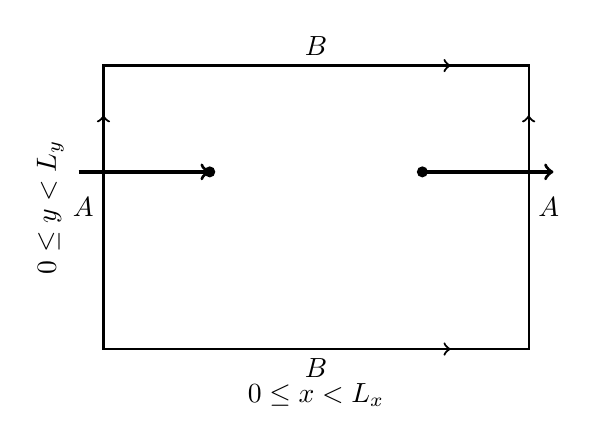
\begin{tikzpicture}[x=0.9cm,y=0.9cm]
\draw[thick] (0,0) rectangle (6,4);
\draw[->,thick] (0,0.7) -- (0,3.3);
\draw[->,thick] (6,0.7) -- (6,3.3);
\draw[->,thick] (1.1,0) -- (4.9,0);
\draw[->,thick] (1.1,4) -- (4.9,4);
\node[left] at (0,2) {$A$};
\node[right] at (6,2) {$A$};
\node[below] at (3,0) {$B$};
\node[above] at (3,4) {$B$};
\draw[->,very thick] (4.5,2.5) -- (6.35,2.5);
\draw[->,very thick] (-0.35,2.5) -- (1.5,2.5);
\fill (4.5,2.5) circle (2pt);
\fill (1.5,2.5) circle (2pt);
\node at (3,-0.65) {$0\leq x<L_x$};
\node[rotate=90] at (-0.75,2) {$0\leq y<L_y$};
\end{tikzpicture}
\caption{Двумерное периодическое пространство: края с одинаковой меткой отождествляются, поэтому частица, пересекающая один край, вновь появляется в соответствующей точке противоположного края.}
\end{figure}

\begin{classroomqa}
\lecturetimestamp{01:50:58}
\audiencequestion{Периодическая конструкция представляет пространство или объекты в пространстве?}
\lecturerresponse{Она представляет пространство. Объекты и поля живут в этом пространстве и подчиняются его отождествлениям. Периодичность вводится, чтобы контролировать проблему бесконечного объёма; затем от неё отказываются, переходя к большому объёму и заменяя суммы по импульсам интегралами.}
\end{classroomqa}

Трёхмерный аналог — это куб с тремя парами отождествлённых противоположных граней. Левая и правая грани одинаковы, верхняя и нижняя одинаковы, и передняя и задняя одинаковы. Частица, пересекающая любую грань, вновь появляется через отождествлённую с ней грань.\footnote{Периодический куб и его три пары отождествлённых противоположных граней показаны в 01:51:27--01:52:17. Приведённое уравнение для \(k_i\) представляет собой покомпонентное восстановление более раннего условия \(kL=2\pi n\), применённого к трём периодическим направлениям.} Три компоненты импульса удовлетворяют
\begin{equation}
k_i=\frac{2\pi n_i}{L_i},
\qquad i=x,y,z,
\end{equation}
где каждому направлению соответствует одно целое число \(n_i\). Торы можно определить в любом числе измерений по тому же правилу.

\begin{figure}[t]
\centering
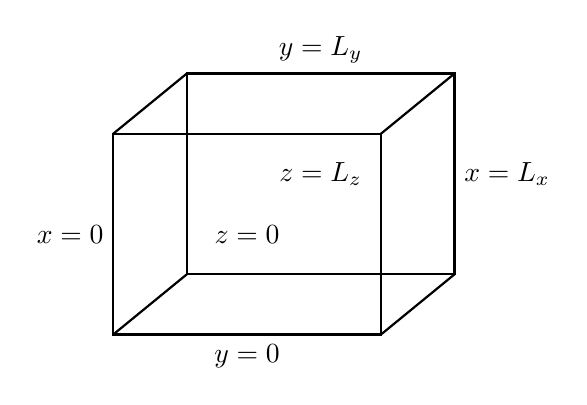
\begin{tikzpicture}[scale=0.85]
\draw[thick] (0,0) rectangle (4,3);
\draw[thick] (1.1,0.9) rectangle (5.1,3.9);
\draw[thick] (0,0) -- (1.1,0.9);
\draw[thick] (4,0) -- (5.1,0.9);
\draw[thick] (4,3) -- (5.1,3.9);
\draw[thick] (0,3) -- (1.1,3.9);
\node[left] at (0,1.5) {$x=0$};
\node[right] at (5.1,2.4) {$x=L_x$};
\node[below] at (2,0) {$y=0$};
\node[above] at (3.1,3.9) {$y=L_y$};
\node at (2,1.5) {$z=0$};
\node at (3.1,2.4) {$z=L_z$};
\end{tikzpicture}
\caption{Трёхмерное периодическое пространство как куб, в котором каждая пара противоположных граней отождествлена.}
\end{figure}

\begin{classroomqa}
\lecturetimestamp{01:52:20}
\audiencequestion{Задаёт ли теория поля физический шаг пространственной решётки?}
\lecturerresponse{Это спекулятивный вопрос. Для практических целей здесь пространство непрерывно. Кванты — это частицы, а не ячейки пространственной решётки. В построении на окружности дискретным становится именно импульс; положение остаётся непрерывным и периодическим.}
\end{classroomqa}

\editorialnote{В длинном повреждённом фрагменте обсуждения шага решётки упоминаются планковские масштабы, но в нём не сохранилось поддающегося восстановлению утверждения о фундаментальной дискретности пространства. Поэтому здесь никакого такого утверждения не выводится.}

Дискретность \(k\) возникла исключительно из-за наложения периодичности на волновую функцию. Это не свидетельствует о том, что сама координата \(x\) лежит на решётке. Вопрос о том, может ли пространство иметь фундаментальную микроскопическую структуру, правомерен, но это отдельный спекулятивный вопрос.

\section{Фермионы и внешние поля}

Для бозонных мод допустимо любое неотрицательное число заполнения. Для фермионов имеет место противоположное поведение: принцип запрета Паули запрещает двум тождественным фермионам занимать одно и то же состояние.

\begin{classroomqa}
\lecturetimestamp{01:55:13}
\audiencequestion{Дает ли замена коммутаторов антикоммутаторами простейшую теорию фермионов?}
\lecturerresponse{Да, по существу. Коммутатор — это \([A,B]=AB-BA\), тогда как антикоммутатор — это \(\{A,B\}=AB+BA\). Соответствующая фермионная алгебра операторов рождения и уничтожения реализует принцип запрета Паули: второго тождественного фермиона нельзя поместить в уже занятое состояние. Подробное изложение теории откладывается.}
\end{classroomqa}

Эти два произведения различаются знаком:
\begin{equation}
[A,B]=AB-BA,
\qquad
\{A,B\}=AB+BA.
\end{equation}
Коммутатор антисимметричен относительно перестановки, тогда как антикоммутатор симметричен. Если антикоммутатор равен нулю, то
\begin{equation}
\{A,B\}=0
\quad\Longrightarrow\quad
AB=-BA.
\end{equation}
Для такой пары перестановка двух фермионных операторов меняет знак. Это необычнее, чем обычное коммутирование, при котором \([A,B]=0\) влечёт \(AB=BA\). Замена бозонных коммутаторов соответствующей антикоммутирующей алгеброй — это математическое изменение, приводящее к фермионам; его подробное развитие отложено.

Антикоммутация обращает статистическое поведение, характерное для бозонов. Здесь нет стимулированного накопления тождественных фермионов в одной моде; заполнение этой моды не позволяет другому тождественному фермиону попасть в неё. Поскольку одно фермионное состояние может содержать не более одного тождественного фермиона, классический полевой предел не получается, если поместить сколь угодно большое их число в это одно состояние.

\begin{classroomqa}
\lecturetimestamp{01:58:03}
\audiencequestion{Как может альфа-частица быть бозоном, если она состоит из фермионов?}
\lecturerresponse{Связанная составная система, содержащая чётное число фермионных составляющих, может обладать бозонной статистикой. Поместить несколько таких составных бозонов в одно и то же общее состояние — не то же самое, что поместить составляющие их отдельные фермионы в одно и то же тождественное одночастичное состояние.}
\end{classroomqa}

Статистика составной системы относится к связанному объекту в целом. Поэтому фермионные составляющие могут объединяться в объект, который ведёт себя как бозон, не нарушая принципа запрета для самих составляющих.

\begin{classroomqa}
\lecturetimestamp{01:58:33}
\audiencequestion{Как учитываются внешние поля?}
\lecturerresponse{До сих пор в построение не включалось никакое внешнее фоновое поле. Такое поле можно задать как классическое поле или представить квантово-механически состоянием, содержащим большое число квантов.}
\end{classroomqa}

Чтобы эти два описания согласовывались, состояние с большим числом заполнения должно быть приготовлено надлежащим образом и быть фазово-когерентным; одного лишь числа частиц недостаточно.\footnote{В обсуждении задаётся масштаб большого числа квантов. Фазовая когерентность сформулирована здесь как дополнительное условие, не позволяющее принять одно лишь большое заполнение за классическое поле.} В этом полуклассическом режиме их эффекты совпадают с точностью до малых квантовых отклонений. Это базовое условие согласованности. Электромагнитное поле должно описывать дискретные фотоны, когда важны отдельные кванты, и вместе с тем должным образом фазово-когерентное состояние, содержащее много фотонов, должно воспроизводить привычное действие классической электромагнитной волны.
